\section{字节码转换框架}
Codger解析器加载源程序时,前先对源程序进行词法分析,词别出由字符序列组成的单词,接着把单词交给语法分析模块处理。语法分析模块会生与源程序等价的抽象语法树,交给字节码转换模块。字节码转换模块负责根据抽象语法树生成字节码。

抽象语法树(abstract syntax tree,AST)是源代码的抽象语法结构的树状表示,它并不依赖于源语言的语法,树上的每个节点都表示源代码中的一种结构,这所以说是抽象的,是因为抽象语法树并不会表示出真实语法出现的每一个细节,比如说,嵌套括号被隐含在树的结构中,并没有以节点的形式呈现。

Codger字节码转换算法采递归的形式把抽象语法树转换成字节码。语法树的每个节点实现了方法getopocde,当父节点getopcode方法被调用时,它会依次调用子节点的getopcode方法得到子节点的字节码,最后把所有子节点的字节码加工后返回。例如:a+b*c生成抽象语法后(如图\ref{fig:abs_tree2})得到根节点root,根节点root指向节点plus,节点plus有两个子节点,左节点为variable\_a,右节点为mul。当plus的 getopcode 被调用时,plus会先调用左节点variable\_a的 getopcode 方法得到左节点的字节码,然后调用右节点mul的 getopcode 方法得到右节点的字节码,最后把两个字节码加在一起,在后面增加一条OP\_PLUS,如下图:
\begin{quote}
\begin{verbatim}
+-----------+--------------+-------+
|左节点字节码| 右节点字节码 |OP_PLUS|
+ ----------+--------------+-------+
\end{verbatim}
\end{quote}
每种类型的节点有3种不同类型的转换:取值转换,赋值转换,运算并赋值转换。
\begin{enumerate}
\item 取值转换表示取当前节点的值,也就是上面谈到的getopcode方法,每个节点必须实现这种转换方式。
\item 赋值转换用于直接赋值语句中,表示对该节点赋值,这种转换方式为可选。例如:语句 a=a 生成抽象语法树后有两个节点,虽然左节点和右节点的类型相同,但它们的转换方式却不同,左节点赋值转换,右节点却为取值转换。
\item 运算并赋值转换转换,用于运算并赋值语句中,这种转换方式为可选。
\end{enumerate}
在实现在算法时,为了尽量减少动态内存的分配,每次先分配一块大的内存,该内存在转换时被所有的节点共享,父节点告诉子节点从那里开始写入它的转换后的字节码,这种方法能提高整个转换算法性能,这也时Codger采用的方法。
\begin{figure}
 \centering
 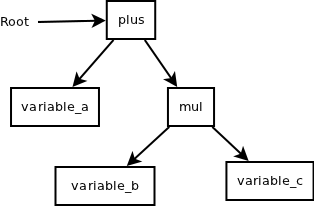
\includegraphics[scale=1]{abs_tree2.png}
 \caption{抽象语法树 a+b*c}
 \label{fig:abs_tree2}
\end{figure}

下面的部分会依次介始每一种类型的节点,它转换字节码的框架。被\verb|<  >|的内容表示这是一个节点,例如图\ref{fig:abs_tree2}节点plus,它有两个子节点,在表示时用\verb|<节点名>|,为了保持整体的可读性,一条语句的所有信息都会出现。节点plus用后面的表示法为:
\begin{quote}
\begin{verbatim}
<expr1> + <expr2> 
\end{verbatim}
\end{quote}
其中\verb|<expr1>|表示左节点,\verb|<expr2>|表示右节点,它被转换后的字节码表示为:
\begin{quote}
\begin{verbatim}
{
    expr1
}
{
    expr2
}
OP_PLUS
\end{verbatim}
\end{quote}
大括号表示调用子节点的getopcode方法。从上到下表示转换过后的字节码的排列顺序,节点expr1排在最前面,所以它在上面,最以OP\_PLUS结尾。

\subsection{常量}
\noindent常量用LITERAL表示,转换成字节码为:
\begin{quote}
\begin{verbatim}
OP_LOAD_CONST $(id)
\end{verbatim}
\end{quote}
其中
\begin{quote}
id=MayConst(LITERAL)
\end{quote}
MapConst把LITERAL放入常量池中,并返回索引该LITERAL的id号。常量池是一位数组,id号是在数组中存LITERAL的位置。

\subsection{变量}
\begin{enumerate}
\item 获当前作用的变量identifier,转换成字节码为:
\begin{quote}
\begin{verbatim}
OP_LOAD_SYMBOL $(id)
\end{verbatim}
\end{quote}
其中
\begin{quote}
id=MaySymbol(identifier)
\end{quote}
MapSymbol把identifier放入符号池中,并返回索引该identifier的id号。符号池是一位数组,id号是在数组中存identifier的位置。

\item 在上层作用域查找变量,如果上层作用域没有找到该变量,则到上层的上层作用域中查找,并依次下去,语句形式:
\begin{quote}
\verb|$identifier|
\end{quote}
转换在字节码为:
\begin{quote}
\begin{verbatim}
OP_LOAD_U_SYMBOL $(id)
\end{verbatim}
\end{quote}
其中
\begin{quote}
id=MaySymbol(identifier)
\end{quote}
\end{enumerate}

\subsection{数组}
\noindent语句形式:
\begin{quote}
\begin{verbatim}
[ <expr1>, ... , <exprn> ]
\end{verbatim}
\end{quote}
省略号表示expr节点类型有n(\verb|n>=0|)个,n的值需要根据源程序来能确定,转换成字节码为:
\begin{quote}
\begin{verbatim}
OP_ARRAY_BEGIN
{
    expr1
}
OP_ARRAY_PUSH
   ...
{
    exprn
}
OP_ARRAY_PUSH
\end{verbatim}
\end{quote}

\subsection{散列表}
\noindent语句形式:
\begin{quote}
\begin{verbatim}
{ <expr_key1> -> <expr_value1> , ... ,<expr_keyn> -> <expr_valuen> } 
\end{verbatim}
\end{quote}
其中\verb|n>=0|,转换成字节码为:
\begin{quote}
\begin{verbatim}
OP_HASH_BEGIN
{
    expr_value1
}
{
    expr_key1
}
OP_HASH_MAP
    ...
{
    expr_valuen
}
{
    expr_keyn
}
OP_HASH_MAP
\end{verbatim}
\end{quote}




\subsection{一元运算符}
\noindent语句形式:
\begin{quote}
\begin{verbatim}
unary_oper <expr>
\end{verbatim}
\end{quote}
转换成字节码为:
\begin{quote}
\begin{verbatim}
{
    expr
}
OP_$(UNARY_OPER)
\end{verbatim}
\end{quote}
大括号表示需要根据expr的具体类型来转换字节码,\$(UNARY\_OPER)表示变量,它的值根据unary\_oper来确定:
\begin{quote}
1) 当unary\_oper 为 + 时,UNARY\_OPER 的值为 POSITIVE \\
2) 当unary\_oper 为 - 时,UNARY\_OPER 的值为 NEGATIVE \\
3) 当unary\_oper 为 \verb|~| 时,UNARY\_OPER 的值为 NEGATED \\
4) 当unary\_oper 为 not 时,UNARY\_OPER 的值为 LOGIC\_NOT
\end{quote}

\subsection{下标运算符()}
\noindent语句形式:
\begin{quote}
\begin{verbatim}
expr ( <expr1> , ... , <exprn> )  
\end{verbatim}
\end{quote}
其中n\verb|>|=0, 转换成字节码为:
\begin{quote}
\begin{verbatim}
{
    expr
}
OP_ARRAY_BEGIN
{
    expr1
}
OP_ARRAY_PUSH
   ...
{
    exprn
}
OP_ARRAY_PUSH
OP_$(BRACKET)
\end{verbatim}
\end{quote}
其中:
\begin{quote}
\begin{verbatim}
1)当expr以成员访问结束时,例如circle.area(),BRACKET的值为CALL_WITH_HOST
2)其它的情况下,例如 cos(3), BRACKET 的值为 CALL
\end{verbatim}
\end{quote}
\subsection{下标运算符[ ]}
\noindent语句形式:
\begin{quote}
\begin{verbatim}
<expr> [ <expr1> ]
\end{verbatim}
\end{quote}
转换成字节码为:
\begin{quote}
\begin{verbatim}
{
    expr
}
{
    expr1
}
OP_GET_ITEM
\end{verbatim}
\end{quote}

\subsection{下标运算符 . }
\noindent语句形式:
\begin{quote}
\begin{verbatim}
<expr> . <identifier>
\end{verbatim}
\end{quote}
转换成字节码为:
\begin{quote}
\begin{verbatim}
{
    expr
}
OP_GET_ATTR $(id)
\end{verbatim}
\end{quote}
如果运算符 . 号后面紧跟 运算符 () ,则字节码转换为:
\begin{quote}
\begin{verbatim}
{
    expr
}
OP_DUP_DATA1
OP_GET_ATTR $(id)
\end{verbatim}
\end{quote}

其中:
\begin{quote}
id=MapSymbol(identifier)
\end{quote}



\subsection{二元运算符}
\noindent语句形式:
\begin{quote}
\begin{verbatim}
<expr_left> binary_oper <expr_right>
\end{verbatim}
\end{quote}
转换成字节码为:
\begin{quote}
\begin{verbatim}
{
    expr_left
}
{
    expr_right
}
OP_$(BINARY_OPER)

\end{verbatim}
\end{quote}
其中:
\begin{quote}
\begin{verbatim}
1)当binary_oper 为 * 时, BINARY_OPER 的值为 MUL
2)当binary_oper 为 / 时, BINARY_OPER 的值为 DIV 
3)当binary_oper 为 % 时, BINARY_OPER 的值为 MOD 
4)当binary_oper 为 + 时, BINARY_OPER 的值为 PLUS 
5)当binary_oper 为 - 时, BINARY_OPER 的值为 MINUS
6)当binary_oper 为 << 时, BINARY_OPER 的值为 LSHIFT
7)当binary_oper 为 >> 时, BINARY_OPER 的值为 RSHIFT
8)当binary_oper 为 & 时, BINARY_OPER 的值为 AND
9)当binary_oper 为 ^ 时, BINARY_OPER 的值为 XOR
10)当binary_oper 为 | 时, BINARY_OPER 的值为 OR
11)当binary_oper 为 < 时, BINARY_OPER 的值为 LT
12)当binary_oper 为 <= 时, BINARY_OPER 的值为 LE
13)当binary_oper 为 == 时, BINARY_OPER 的值为 EQ
14)当binary_oper 为 != 时, BINARY_OPER 的值为 NE
15)当binary_oper 为 <= 时, BINARY_OPER 的值为 GE
16)当binary_oper 为 < 时, BINARY_OPER 的值为 GT
\end{verbatim}
\end{quote}

\subsection{逻辑运算符AND}
\noindent语句形式:
\begin{quote}
\begin{verbatim}
<expr_left> and <expr_right>
\end{verbatim}
\end{quote}
转换成字节码为:
\begin{quote}
\begin{verbatim}
{
    expr_left
}
OP_DUP_DATA1
OP_JUMPR_FALSE_FORWARD  $(End)
OP_DISCARD
{
    expr_right
}
@label End
\end{verbatim}
\end{quote}
其中\$(End)表示OP\_JUMPR\_FALSE\_FORWARD 跳转的相对地址,@lable End 用于标识指令的位置。

\subsection{逻辑运算符OR}
\noindent语句形式:
\begin{quote}
\begin{verbatim}
<expr_left> or <expr_right>
\end{verbatim}
\end{quote}
转换成字节码为:
\begin{quote}
\begin{verbatim}
{
    expr_left
}
OP_DUP_DATA1
OP_JUMPR_TRUE_FORWARD  $(End)
OP_DISCARD
{
    expr_right
}
@label End
\end{verbatim}
\end{quote}

\subsection{表达式语句}
\noindent语句形式:
\begin{quote}
\verb|<expr>|
\end{quote}
转换成字节码为:
\begin{quote}
\begin{verbatim}
{
    expr
}
OP_DISCARD
\end{verbatim}
\end{quote}

\subsection{直接赋值语句}
赋值语句有左节点和右节点,左节点为被赋值的对象,转换方式为赋值转换;右节点的转换方式为取值转换。
\noindent语句形式:
\begin{quote}
\begin{verbatim}
<expr1> = <expr2>
\end{verbatim}
\end{quote}
转换成字节码为:
\begin{quote}
\begin{verbatim}
{
    expr2
}
{
    expr1
}
\end{verbatim}
\end{quote}
其中expr1为赋值转换,它有下面的几种情况:

\begin{enumerate}
\item 给变量赋值,语句形式:
\begin{quote}
\begin{verbatim}
<identifier> = <expr>
\end{verbatim}
\end{quote}
转换成字节码为:
\begin{quote}
\begin{verbatim}
{
   expr
}
OP_STORE_SYMBOL $(id)
\end{verbatim}
\end{quote}
其中:
\begin{quote}
id=MapSymbol(identifier)
\end{quote}
\item 给上层作用域的变量赋值,如果上层作用域没有找到该变量,则到上层的上层作用域中查找,并依次下去,语句形式:
\begin{quote}
\begin{verbatim}
<$identifier> = <expr>
\end{verbatim}
\end{quote}
转换成字节码为:
\begin{quote}
\begin{verbatim}
{
   expr
}
OP_STORE_U_SYMBOL $(id)
\end{verbatim}
\end{quote}
其中:
\begin{quote}
id=MapSymbol(identifier)
\end{quote}
\item 给集合指令的元素赋值,语句形式
\begin{quote}
\begin{verbatim}
<expr> [ <expr1> ] = <expr2>
\end{verbatim}
\end{quote}
转换成字节码为:
\begin{quote}
\begin{verbatim}
{
    expr2
}
{
    expr  
}
{
    expr1
}
OP_SET_ITEM
\end{verbatim}
\end{quote}
\item 给对象的成员赋值,语句形式
\begin{quote}
\begin{verbatim}
<expr> . <identifier> = <expr1>
\end{verbatim}
\end{quote}
转换成字节码为:
\begin{quote}
\begin{verbatim}
{
    expr1
}
{
    expr  
}
OP_SET_ATTR $(id)
\end{verbatim}
\end{quote}
其中:
\begin{quote}
id=MapSymbol(identifier)
\end{quote}
\end{enumerate}

\subsection{运算并赋值语句}
\noindent运算并赋值语句和赋值语句一样有两上节点,左节点为运算并赋值转换,右节点为取值转换,左节点的类型有以下几种情况:
\begin{enumerate}
\item 变量运算并赋值,语句形式:
\begin{quote}
\begin{verbatim}
<identifier> assign_oper <expr>
\end{verbatim}
\end{quote}
转换成字节码为:
\begin{quote}
\begin{verbatim}
{
    expr 
}
OP_LOAD_SYMBOL  $(id)
OP_DATA_SWAP0_1
OP_$(OPER)
OP_STORE_SYMBOL $(id)
\end{verbatim}
\end{quote}
其中:
\begin{quote}
\begin{verbatim}
id=MapSymbol(identifier)

1)当assign_oper 为 *= 时, OPER 的值为 MUL
2)当assign_oper 为 /= 时, OPER 的值为 DIV 
3)当assign_oper 为 %= 时, OPER 的值为 MOD 
4)当assign_oper 为 += 时, OPER 的值为 PLUS 
5)当assign_oper 为 -= 时, OPER 的值为 MINUS
6)当assign_oper 为 <<= 时,OPER 的值为 LSHIFT
7)当assign_oper 为 >>= 时,OPER 的值为 RSHIFT
8)当assign_oper 为 &= 时, OPER 的值为 AND
9)当assign_oper 为 ^= 时, OPER 的值为 XOR
10)当assign_ope 为 |= 时, OPER 的值为 OR
\end{verbatim}
\end{quote}
\item 当前作用域以上的变量运算并赋值,语句形式:
\begin{quote}
\begin{verbatim}
<$identifier> assign_oper  <expr>
\end{verbatim}
\end{quote}
转换成字节码为:
\begin{quote}
\begin{verbatim}
{
    expr 
}
OP_LOAD_U_SYMBOL  $(id)
OP_DATA_SWAP0_1
OP_$(OPER)
OP_STORE_U_SYMBOL $(id)
\end{verbatim}
\end{quote}
其中:
\begin{quote}
\begin{verbatim}
id=MapSymbol(identifier)
\end{verbatim}
\end{quote}
OPER与assign\_oper的关系见变量的运算并赋值
\item 与集中的指定的元素运算并赋值,语句形式:
\begin{quote}
\begin{verbatim}
<expr> [ <expr1> ] assign_oper <expr2>
\end{verbatim}
\end{quote}
转换成字节码为:
\begin{quote}
\begin{verbatim}
{
    expr2
}
{
    expr 
}
{
    expr1
}
OP_DUP_DATA3
OP_GET_ITEM
OP_DATA_SWAP0_1
OP_$(OPER)
OP_DATA_SWAP0_3
OP_DISCARD
OP_SET_ITEM
\end{verbatim}
\end{quote}
其中OPER 与assign\_oper的关系见变量的运算并赋值。

\item 和对象的成员运算并赋值,语句形式:
\begin{quote}
\begin{verbatim}
<expr> . <identifier> assign_oper <expr1>
\end{verbatim}
\end{quote}
转换成字节码为:
\begin{quote}
\begin{verbatim}
{
    expr1
}
{
    expr 
}
OP_DUP_DATA2
OP_GET_ATTR $(id)
OP_DATA_SWAP0_1
OP_$(OPER)
OP_DATA_SWAP0_2
OP_DISCARD
OP_SET_ATTR $(id)
\end{verbatim}
\end{quote}
其中:
\begin{quote}
\begin{verbatim}
id=MapSymbol(identifier)
\end{verbatim}
\end{quote}
OPER 与assign\_oper的关系见变量的运算并赋值。
\end{enumerate}

\subsection{print语句}
\noindent语句形式:
\begin{quote}
\begin{verbatim}
print <expr1> , ... , <exprn>
\end{verbatim}
\end{quote}
其中\verb|n>=0|,转换成字节码为:
\begin{quote}
\begin{verbatim}
{
    expr1
}
OP_PRINT
   ...
{
    exprn
}
OP_PRINT
OP_PRINT_LN
\end{verbatim}
\end{quote}

\subsection{for语句}
\noindent语句形式:
\begin{quote}
\begin{verbatim}
for <expr> in <expr1>
    <stmts>
end
\end{verbatim}
\end{quote}
转换成字节码为:
\begin{quote}
\begin{verbatim}
{
    expr1
}
OP_ITER
@lable Begin
OP_ITE_NEXT
OP_JUMPR_FORWARD $(End)
{
    expr
}
{
    stmts
}
OP_JUMPR_BACK $(Begin)
@label End
OP_DISCARD 
\end{verbatim}
\end{quote}
其中expr语句为赋值转换,它的几种情况见直接赋值语句部分。最后需要更新stmts中的OP\_BREAK与OP\_CONTINUE指令
\begin{quote}
\begin{verbatim}
Update OP_BREAK to OP_JUMPR_FORWARD $(End)
Update OP_CONTINUE to OP_JUMPR_BACK $(Begin)
\end{verbatim}
\end{quote}



\subsection{while语句}
\noindent语句形式:
\begin{quote}
\begin{verbatim}
while <expr>
    <stmts>
end 
\end{verbatim}
\end{quote}
转换成字节码为:
\begin{quote}
\begin{verbatim}
@label Begin
{
    expr
}
OP_JUMPR_FALSE_FORWARD $(End)
{
    stmts
}
OP_JUMPR_BACK $(Begin)
@label End
\end{verbatim}
\end{quote}
最后需要更新stmts中的OP\_BREAK和OP\_CONTINUE 指令
\begin{quote}
\begin{verbatim}
Update OP_BREAK to OP_JUMPR_FORWARD $(End)
Update OP_CONTINUE to OP_JUMPR_BACK $(Begin)
\end{verbatim}
\end{quote}

\subsection{if-elif-else语句}
\noindent语句形式:
\begin{quote}
\begin{verbatim}
if <expr1>
   <stmts1>
elif <expr2>
   <stmts2>
elif 
    ....
else 
   <stmtsn>
end 
\end{verbatim}
\end{quote}
其中\verb|n>=0|,转换成字节码为:
\begin{quote}
\begin{verbatim}
{
    expr1
}
OP_JUMPR_FALSE_FORWARD $(L1)
{
    stmts1
}
OP_JUMPR_FORWARD $(End)
@label L1
{
    expr2
}
OP_JUMPR_FALSE_FORWARD $(L2)
{
    stmts2
}
OP_JUMPR_FORWARD $(End)
@label L2
    .....

@lable Ln
{
    stmtsn
}
@label End 
\end{verbatim}
\end{quote}
如果else部分不存在,则去掉字节码中stmtsn的部分。

\subsection{break语句}
\noindent语句形式:
\begin{quote}
break
\end{quote}
转换成字节码为:
\begin{quote}
OP\_BREAK 
\end{quote}
指令OP\_BREAK只是用于辅助字节码的生成,它最终会被替换为OP\_JUMPR*

\subsection{continue语句}
\noindent语句形式:
\begin{quote}
continue 
\end{quote}
转换在字节码为:
\begin{quote}
OP\_CONTINUE 
\end{quote}
指令OP\_CONTINUE只是用于辅助字节码的生成,它最终会被替换为OP\_JUMPR*

\subsection{return语句}
\begin{enumerate}
\item return后跟一个表达式,语句形式:
\begin{quote}
\verb|return <expr>|
\end{quote}
转换成字节码为:
\begin{quote}
\begin{verbatim}
{
    expr
}
OP_RETURN
\end{verbatim}
\end{quote}

\item return后不跟表达式,语句形式:
\begin{quote}
return 
\end{quote}
转换成字节码为:
\begin{quote}
OP\_RETURN\_NIL
\end{quote}
\end{enumerate}

\subsection{函数定义语句}
\begin{enumerate}
\item 有名函数,语句形式为:
\begin{quote}
\begin{verbatim}
func <identifier>( <id_simply1>, ... ,<id_simplyn>,
                 <id_def> = <expr1>, ... , <id_defm> = <exprm>,
                 <*id_many> )
      <stmts>
end 
\end{verbatim}
\end{quote}
其中\verb|n>=0,m>=0|, 解析时,根据stmts,参数个类,及参数类型,生成新的字节码 op\_code \\
转换成字节码为:
\begin{quote}
\begin{verbatim}
OP_FUNC_BEGIN $(op_id)
OP_ARRAY_BEGIN
{
    expr1
}
OP_ARRAY_PUSH
   .....
{
    exprm
}
OP_ARRAY_PUSH
OP_FUNC_DEFALUT_ARGS
OP_DUP_DATA1
OP_STORE_SYMBOL  $(name_id)
\end{verbatim}
\end{quote}
其中:
\begin{quote}
\begin{verbatim}
op_id=MapOpcode(op_code) 
name_id=MapSymbol(identifier)
\end{verbatim}
\end{quote}
\item 匿名函数与有名函数的转换过程相同,但少了最后两个 OP\_DUP\_DATA1 与 OP\_STORE\_SYMBOL 指令
\end{enumerate}

\subsection{类定义语句}
\noindent语句形式:
\begin{quote}
\begin{verbatim}
class <identifier> 
    <class_stmt1>
        ...
    <class_stmtn>
end
\end{verbatim}
\end{quote}
其中\verb|n>=0|,
转换成字节码为:
\begin{quote}
\begin{verbatim}
OP_CLASS_BEGIN
{
    class_stmt1
}
   .....
{
    class_stmtn
}
OP_STORE_SYMBOL $(id)
\end{verbatim}
\end{quote}
其中:
\begin{quote}
id=MapSymbol(identifier)
\end{quote}
class\_stmt有以下几种形式:
\begin{enumerate}
\item 属性申明语句(不带默认值):
\begin{quote}
\begin{verbatim}
<perm> <static> attr <identifier> 
\end{verbatim}
\end{quote}
转换成字节码为:
\begin{quote}
\begin{verbatim}
OP_LOAD_NIL
OP_CLASS_$(TEMP) $(id)
\end{verbatim}
\end{quote}
其中::
\begin{quote}
\begin{verbatim}
id=MapPermSymbol(identifier,perm)
1)如果static不存在,则TEMP=TEMPLATE
2)如果static存在,则TEMP=ATTR
\end{verbatim}
\end{quote}
perm的值为可以为public,protected,private;如果在申明时没说明权限, perm 默认为protected。 MapPermSymbol 把 identifier 放入带权限的符号池中,在identifier 中保存权限信息,并返回索引该 identifier 的 id 号。带权限的符号池是一位数组,id号是在数组中存 identifier 的位置。


\item 属性申明语句(带默认值):
\begin{quote}
\begin{verbatim}
<perm> <static> attr <identifier>  = <expr>
\end{verbatim}
\end{quote}
转换成字节码为:
\begin{quote}
\begin{verbatim}
{
    expr
}
OP_CLASS_$(TEMP) $(id)
\end{verbatim}
\end{quote}
其中:
\begin{quote}
\begin{verbatim}
id=MapPermSymbol(identifier,perm)
1)如果static不存在,则TEMP=TEMPLATE
2)如果static存在,则TEMP=ATTR
\end{verbatim}
\end{quote}


\item 方法申明语句:
\begin{quote}
\begin{verbatim}
<perm> <static> func <identifier>( <id_simply1>, ... ,<id_simplyn>,
                 <id_def> = <expr1>, ... , <id_defm> = <exprm>,
                 <*id_many> )
      <stmts>
end 
      
\end{verbatim}
\end{quote}
其中\verb|n>=0,m>=0|, 解析时,根据stmts,参数个类,及参数类型,生成新的字节码 op\_code \\
转换成字节码为:
\begin{quote}
\begin{verbatim}
OP_FUNC_BEGIN $(op_id)
OP_ARRAY_BEGIN
{
    expr1
}
OP_ARRAY_PUSH
   .....
{
    exprm
}
OP_ARRAY_PUSH
OP_FUNC_DEFALUT_ARGS
OP_CLASS_$(TEMP)  $(name_id)
\end{verbatim}
\end{quote}
其中:
\begin{quote}
\begin{verbatim}
name_id=MapPermSymbol(identifier , perm)
op_id=MapOpcode(op_code) 
1)如果static不存在,则TEMP=TEMPLATE
2)如果static存在,则TEMP=ATTR
\end{verbatim}
\end{quote}
\end{enumerate}

\subsection{import语句}
\begin{enumerate}
\item 语句形式:
\begin{quote}
\begin{verbatim}
import <identifier1> . ~~~ . <identifiern>
\end{verbatim}
\end{quote}
由于省略号与点号会混淆,所以用\verb|~~~|中当存在多个标识符,其中\verb|n>=1| \\
转换成字节码为:
\begin{quote}
\begin{verbatim}
OP_IMPORT $(idx)
OP_STORE_SYMBOL $(id1)
\end{verbatim}
\end{quote}
其中:
\begin{quote}
\begin{verbatim}
idx=MapSymbol(identifier1.~~~.identifiern)
id1=MapSymbol(identifier)
\end{verbatim}
\end{quote}

\item 语句形式:
\begin{quote}
\begin{verbatim}
import <identifier1> . ~~~ . <identifiern> as <identifierm>
\end{verbatim}
\end{quote}
其中\verb|n>=1|, 转换成字节码为:
\begin{quote}
\begin{verbatim}
OP_IMPORT $(idx)
OP_STORE_SYMBOL $(idm)
\end{verbatim}
\end{quote}
其中:
\begin{quote}
\begin{verbatim}
idx=MapSymbol(identifier1.~~~.identifiern)
idm=MapSymbol(identifierm)
\end{verbatim}
\end{quote}
\end{enumerate}

\subsection{export语句}
\begin{enumerate}
\item 语句形式:
\begin{quote}
\begin{verbatim}
export <identifier>
\end{verbatim}
\end{quote}
转换成字节码为:
\begin{quote}
\begin{verbatim}
OP_LOAD_SYMBOL $(id)
OP_EXPORT $(id)
\end{verbatim}
\end{quote}
其中:
\begin{quote}
\begin{verbatim}
id=MapSymbol(identifier) 
\end{verbatim}
\end{quote}

\item 语句形式:
\begin{quote}
\begin{verbatim}
export <expr>  as <identifier>
\end{verbatim}
\end{quote}
转换成字节码为:
\begin{quote}
\begin{verbatim}
{
    expr
}
OP_EXPORT $(id)
\end{verbatim}
\end{quote}
其中:
\begin{quote}
\begin{verbatim}
id=MapSymbol(identifier) 
\end{verbatim}
\end{quote}

\end{enumerate}
